
\section{Discord}

\subsection{Скриншоты}

\begin{center}

    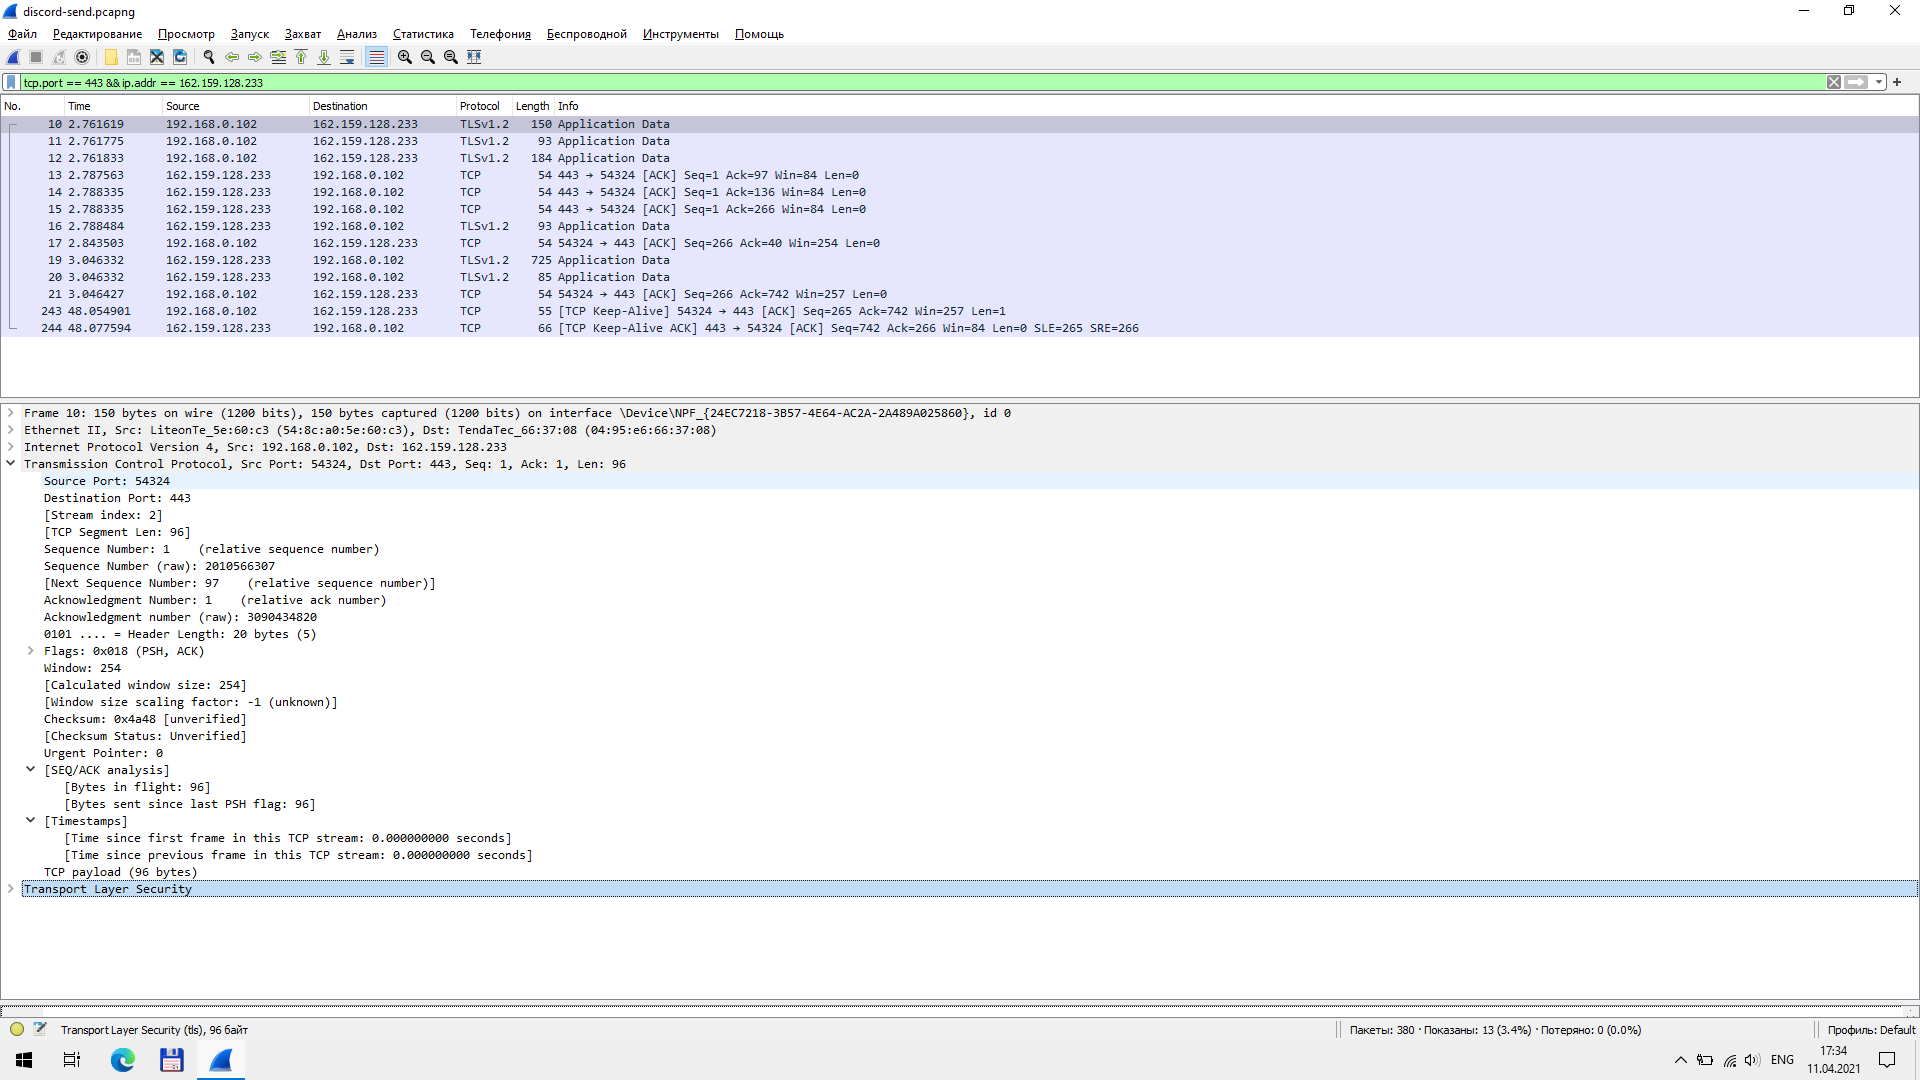
\includegraphics[width=\textwidth]{screenshots/discord_send_1}

    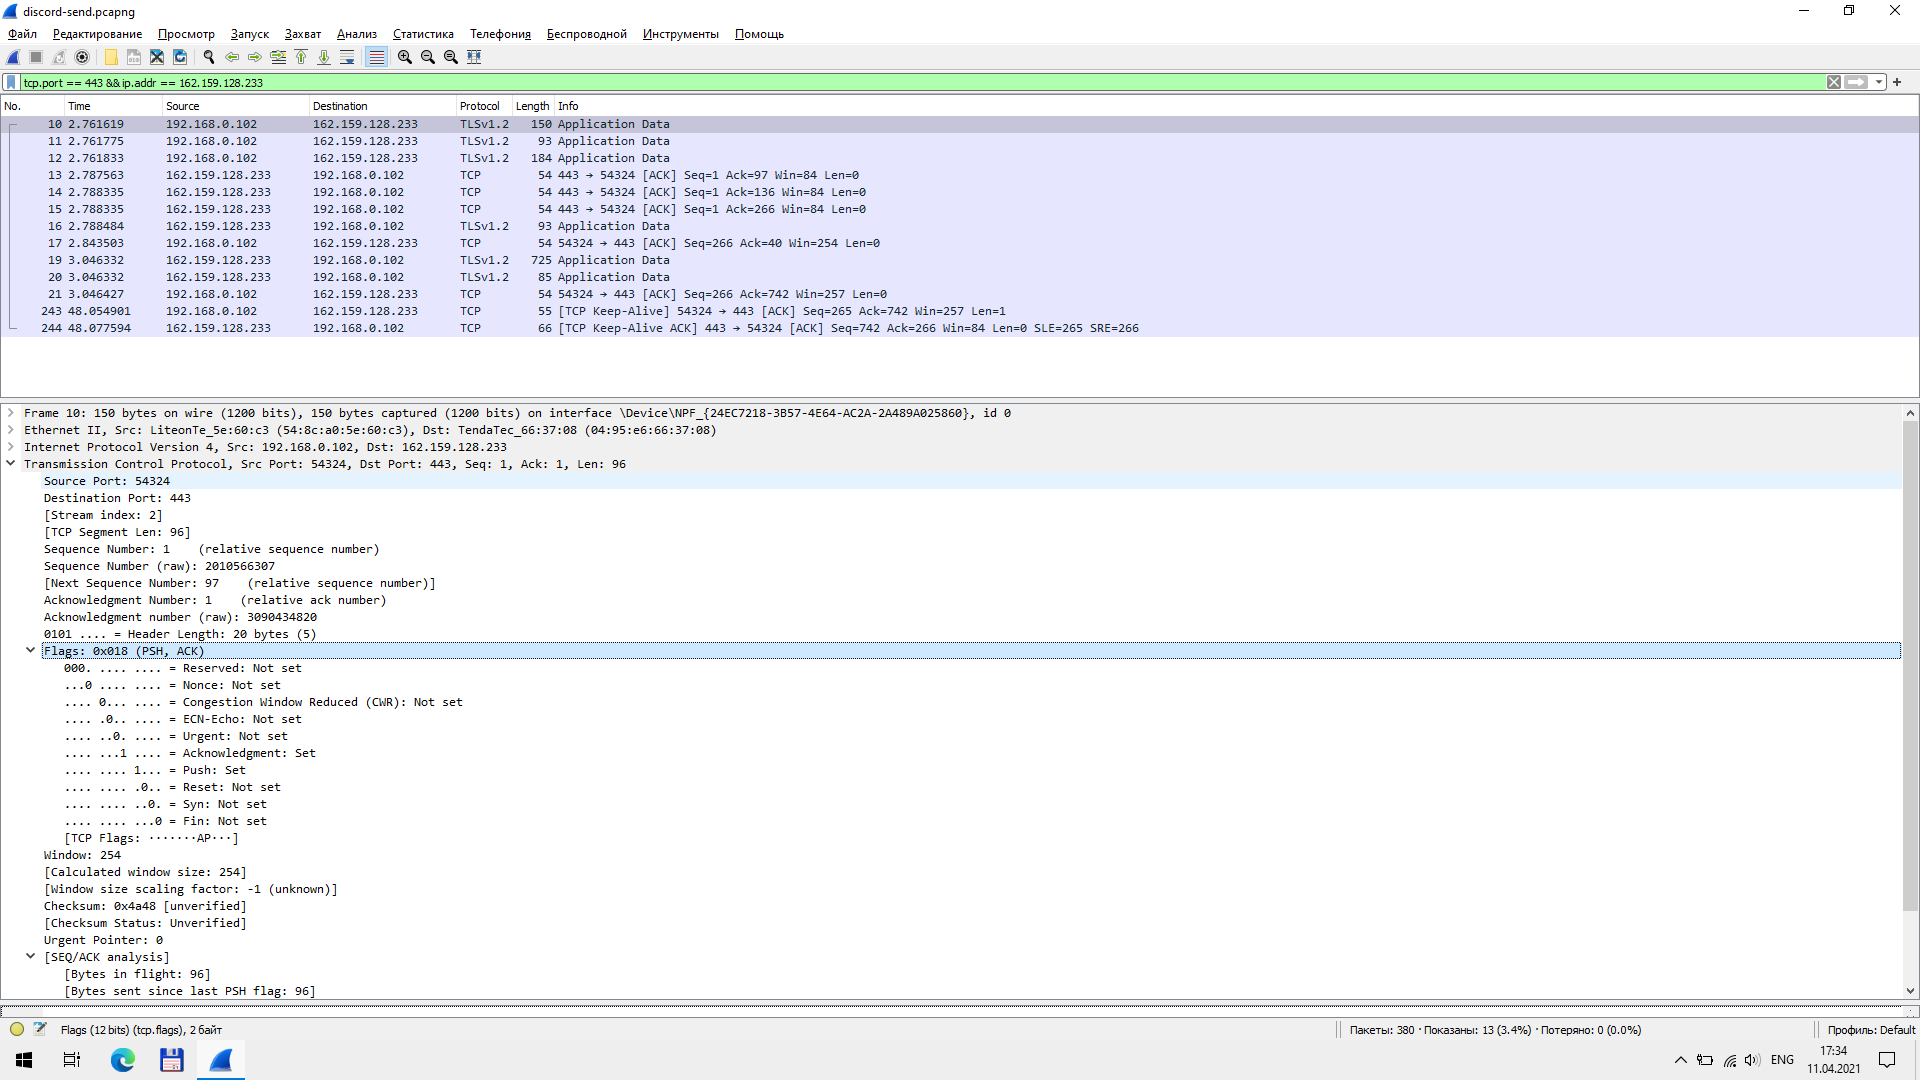
\includegraphics[width=\textwidth]{screenshots/discord_send_2}

    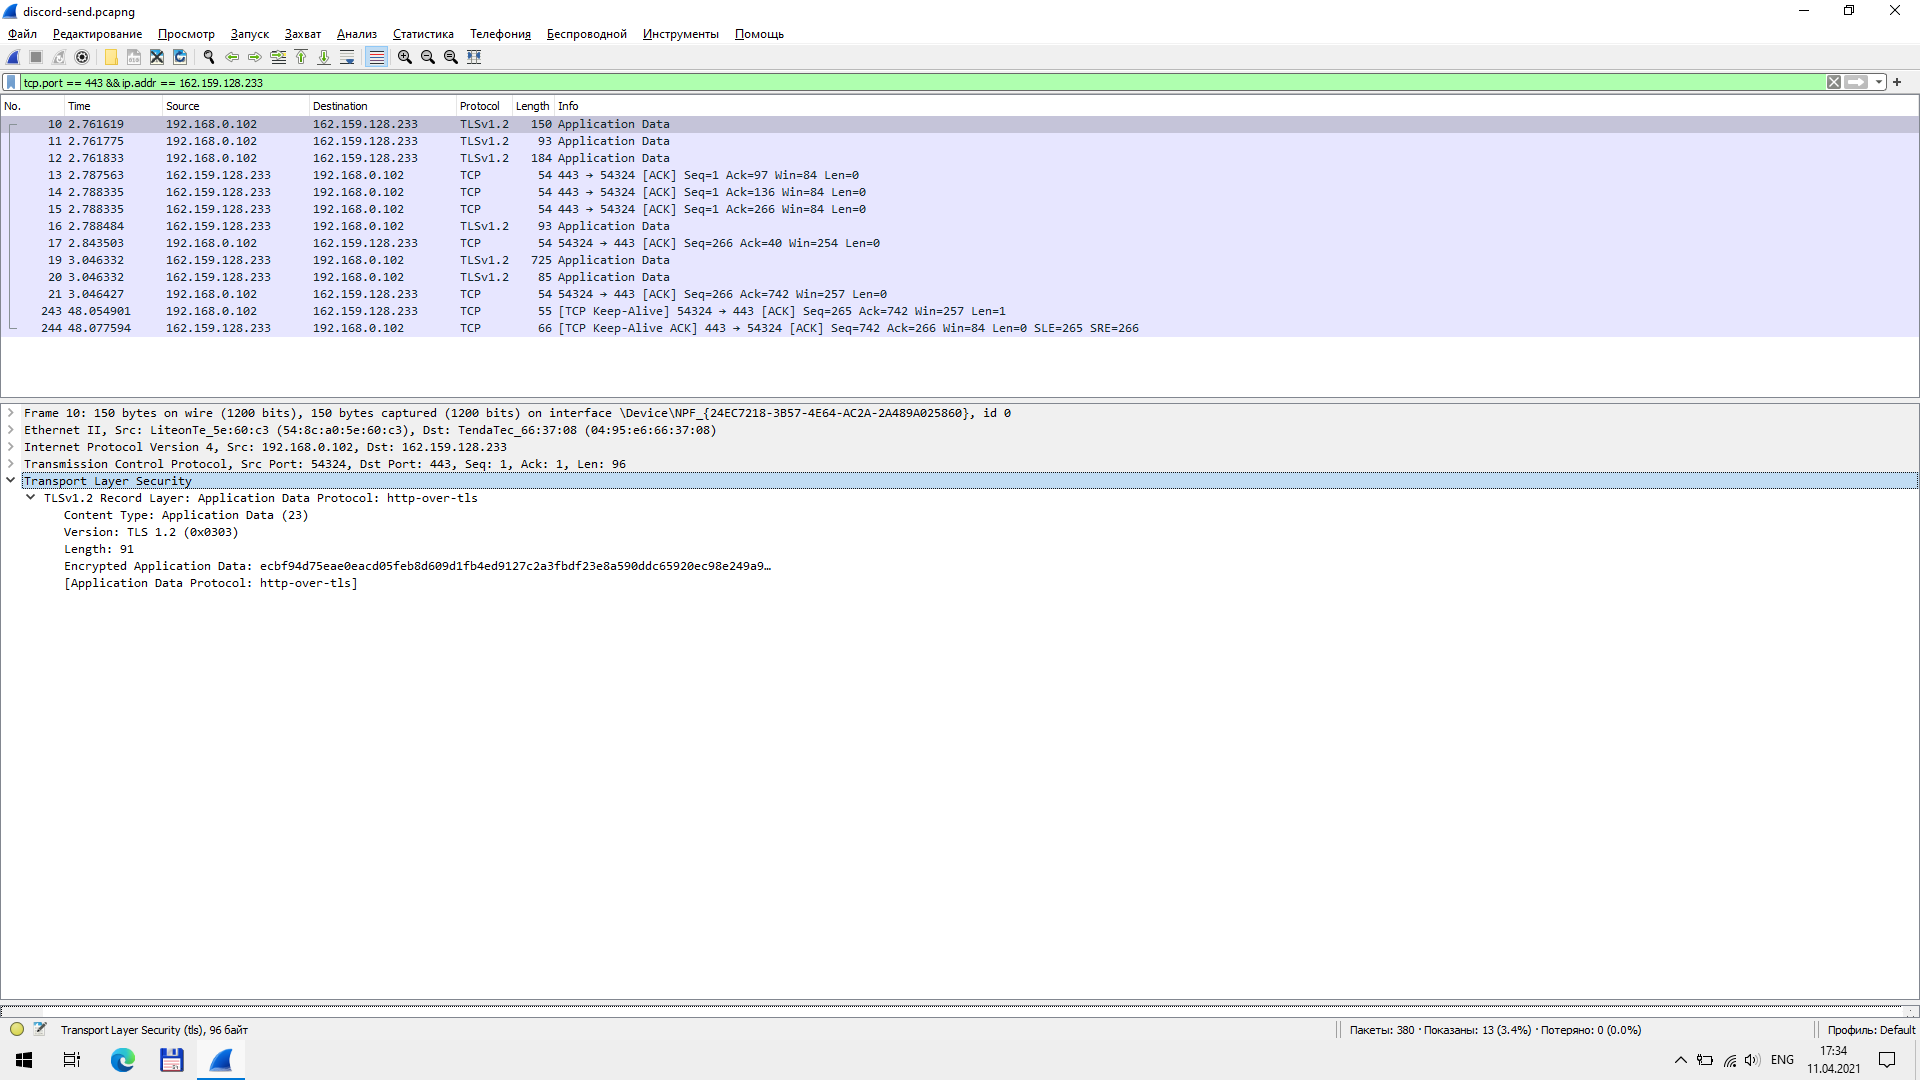
\includegraphics[width=\textwidth]{screenshots/discord_send_3}

    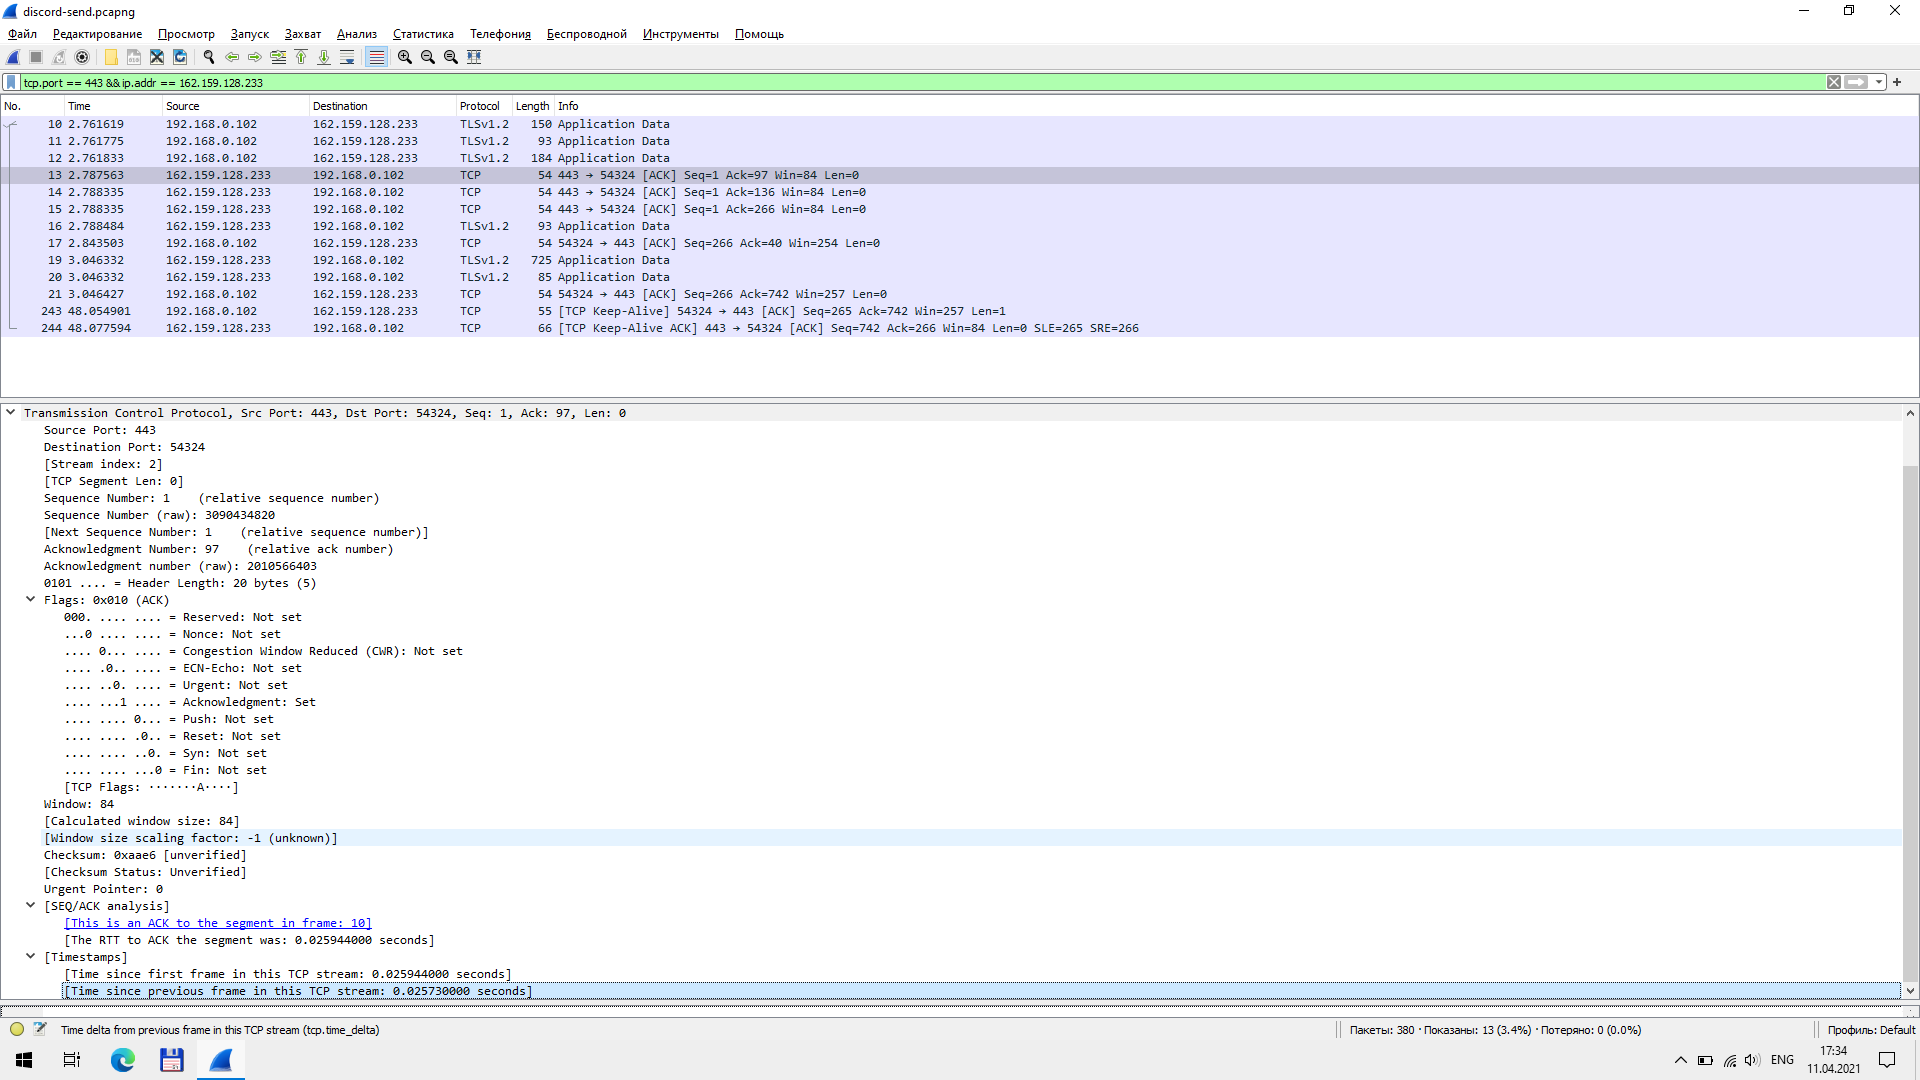
\includegraphics[width=\textwidth]{screenshots/discord_send_4}

    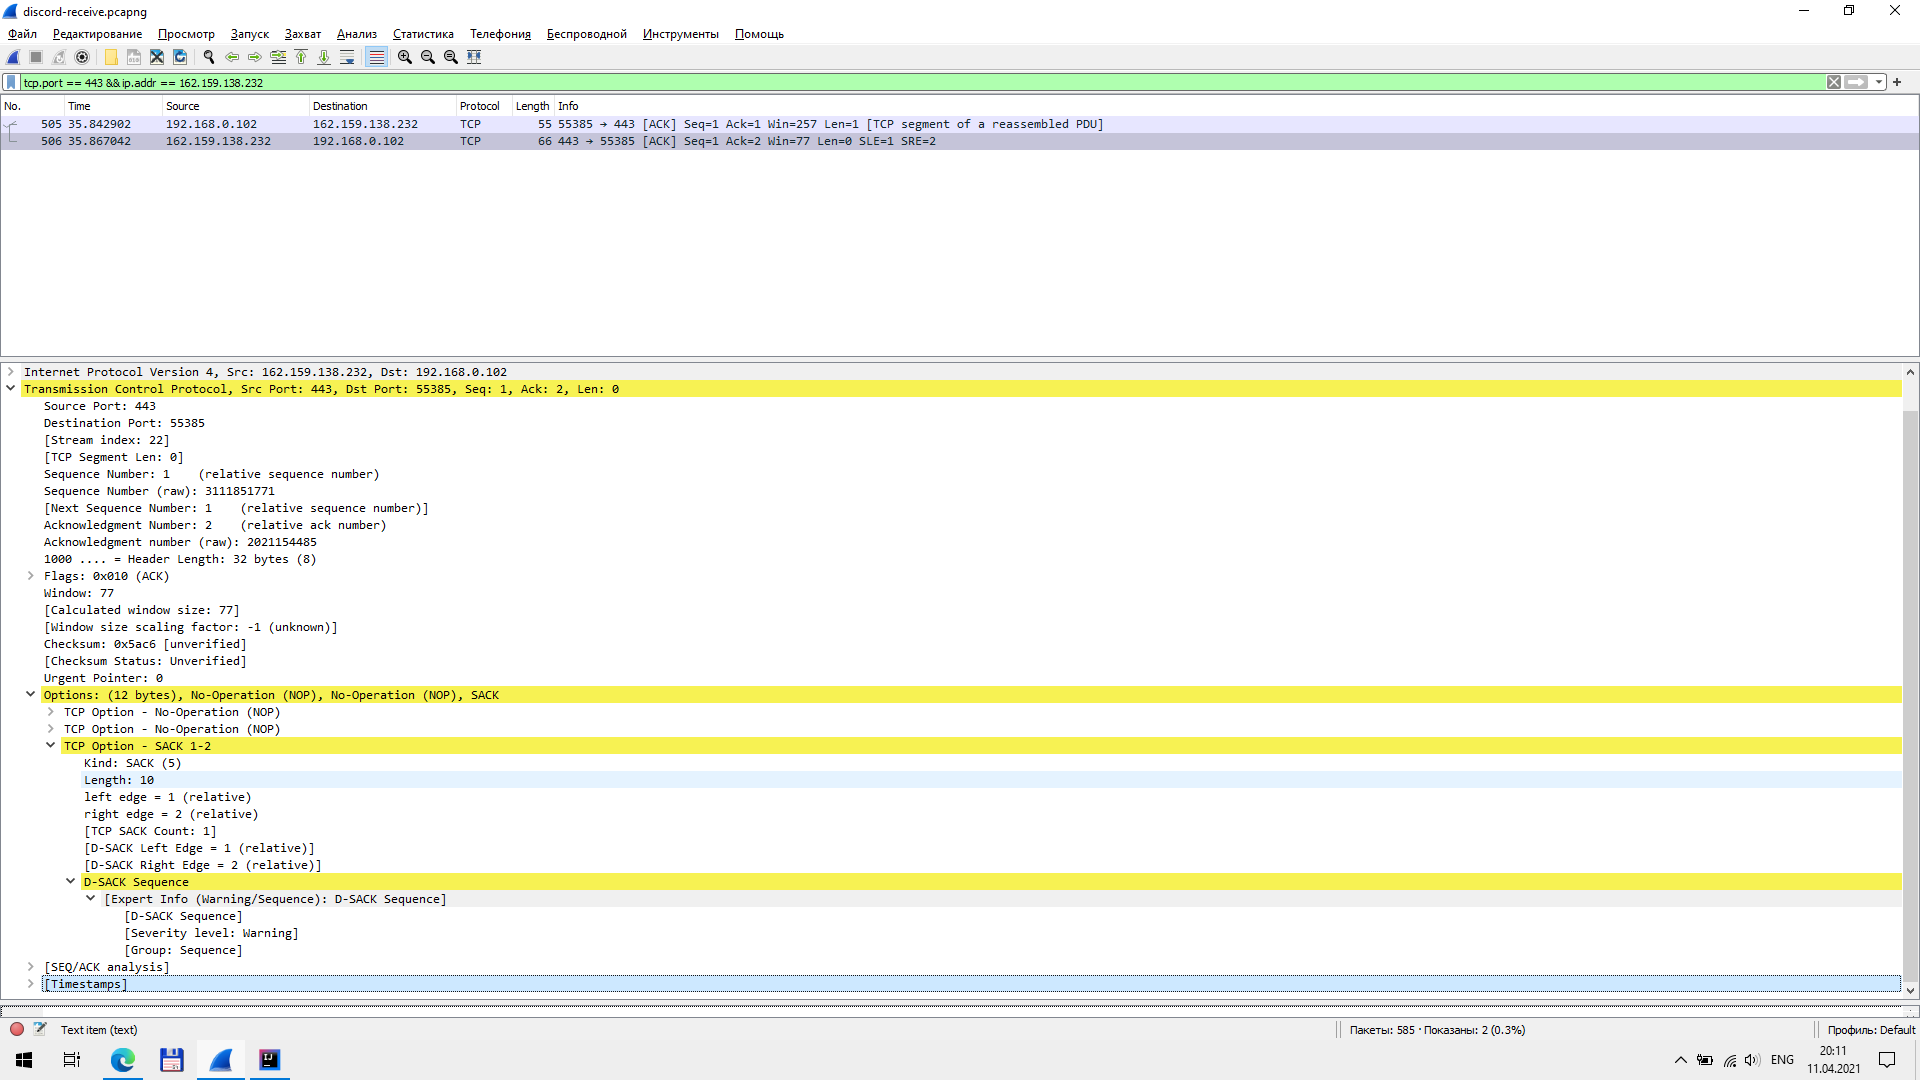
\includegraphics[width=\textwidth]{screenshots/discord_receive_1}

    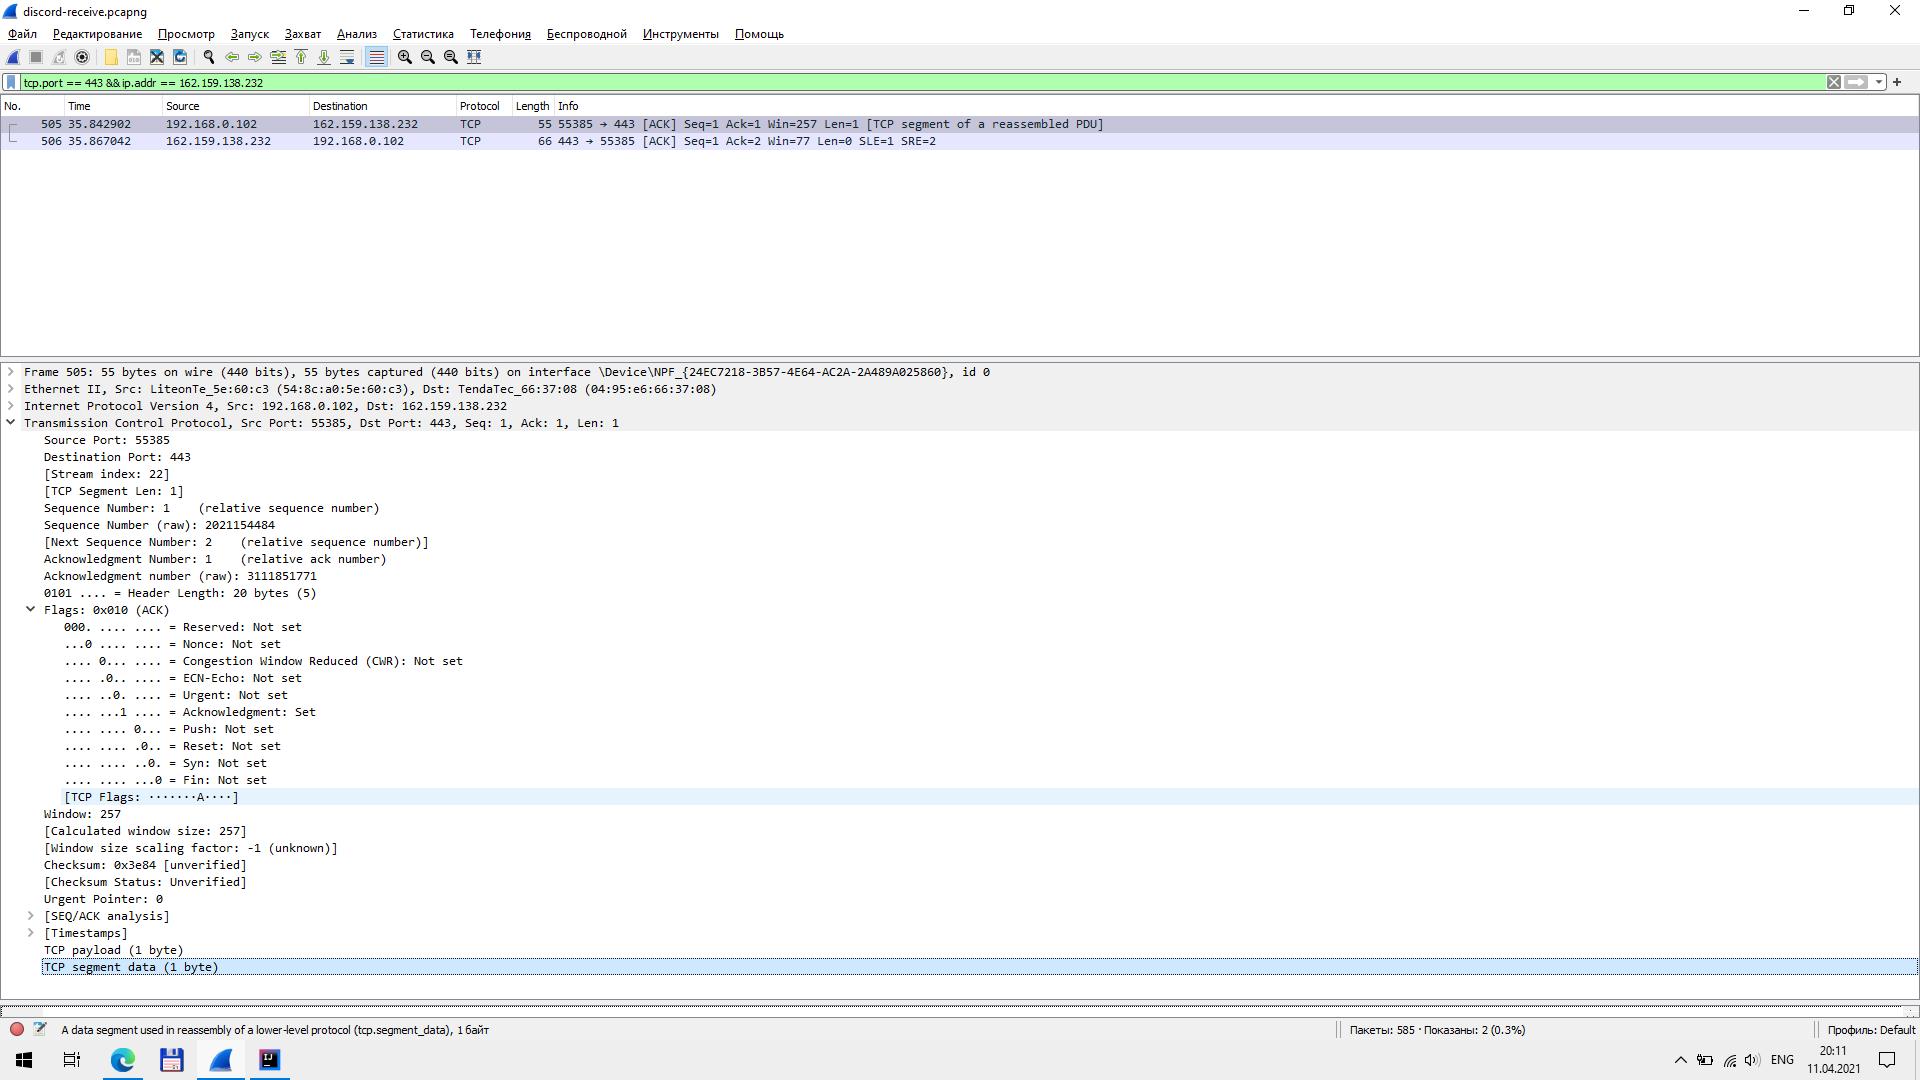
\includegraphics[width=\textwidth]{screenshots/discord_receive_2}

\end{center}

Скриншоты для звонка и видеозвонка принципиально не отличаются,
т.к. тоже представляют из себя зашифрованный TLS-трафик.

\subsection{Ответы на вопросы}

\subsubsection{}
Они отличаются количественно, но т.к. трафик зашифрован, то вытянуть больше информации из Wireshark не получится.

\subsubsection{}
В случае Discord это невозможно по нескольким причинам:
\begin{itemize}
    \item Трафик зашифрован, поэтому отличить текст от аудио/видео можно только количественно.
    \item Аудио и видео передаются по одному и тому же протоколу.
\end{itemize}

Можно только отличить запросы на домен \texttt{discord.com},
даже не на IP-адрес, т.к. он меняется при перезапуске приложения:
есть множество физически разных серверов в разных регионах с одним и тем же доменным именем,
и конкретный сервер выбирается при подключении.
